\documentclass[a4paper,12pt]{article}

\usepackage[top=3cm, bottom=2cm, left=3cm, right=2cm]{geometry}
\usepackage[utf8]{inputenc}
\usepackage[portuguese]{babel}
\usepackage{booktabs}
\usepackage{multirow}
\usepackage{hyperref}
\usepackage{graphicx}
\usepackage{longtable}
\usepackage{verbatim}

\usepackage{float}
\floatstyle{ruled}
\newfloat{program}{thp}{lop}
\floatname{program}{Script}

\title{Serviços de Rede e de Sistema \\
Interior Routing }

\author{André Fernandes (ei03107) \and Miguel Gomes (ei07075) \and Pedro Batista (ext10392)}

\begin{document}

\maketitle

\section{Topologia}
A topologia de rede implementada foi exatamente igual à proposta do relatório. Esta é mostrada na Figura~\ref{fig:topologia}.

\begin{figure}[htp]
	\begin{center}
		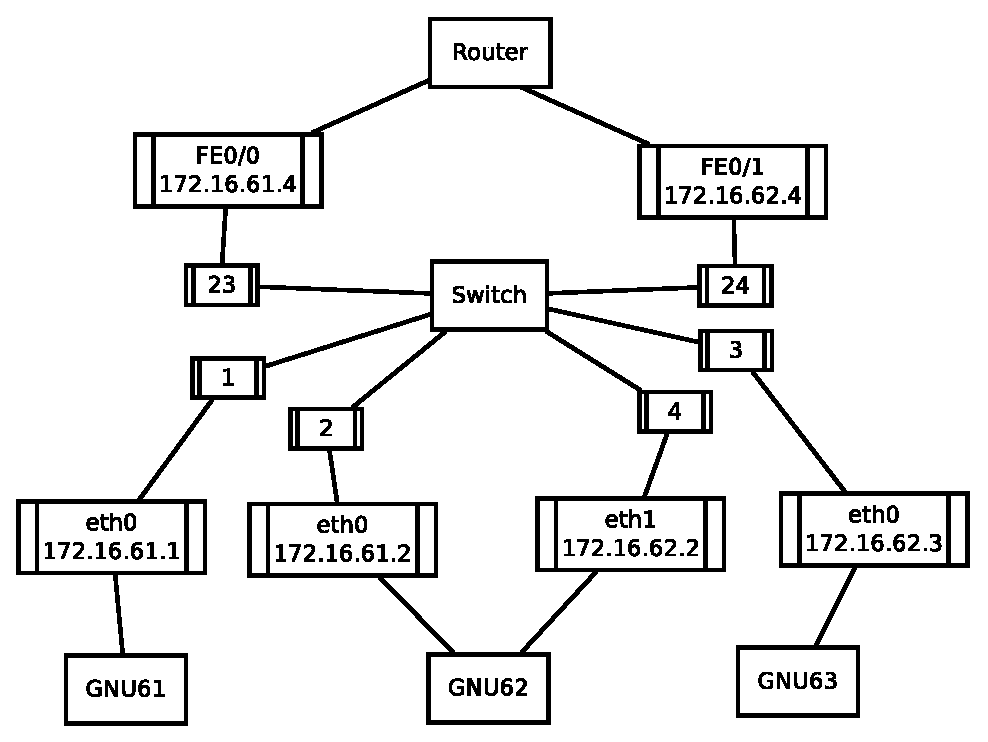
\includegraphics[height=4in]{topologia}
	\end{center}
	\caption{Topologia de rede implementada.}
	\label{fig:topologia}
\end{figure}

\section{Cenários}

	De acordo com o especificado no trabalho foram implementados e estudados 3 cenários distintos. Para cada um deles foram executados os vários testes pedidos, para além de análise de tráfego e geração de ficheiros de logs, que serão explicados nas secções seguintes.
		
	O primeiro cenário consiste numa implementação simples da topologia referida acima, sem forçar custos por rota nem designações de DR/BDR. Para este cenário apenas era pedido que fosse verificada a conexão entre os vários GNUs, para além de análise de tráfego e logs do zebra e ospf, sendo obtidos os resultados esperados.
			
	No segundo cenário foi novamente respeitada a topologia referida acima, tendo apenas sido forçado o DR para o GNU62 e o BDR para o router em cada uma das redes. Também foram modificadas as configurações de BW, de forma a que o caminho entre o GNU61 e o GNU63 tivesse o mesmo custo quer passasse pelo GNU62 ou pelo router. Para além dos testes referidos no cenário anterior foram também efectuados vários trace routes para verificar o caminho dos pacotes por cada ligação, especialmente na ligação entre o GNU61 e o GNU63, onde se verificou que foram escolhidos os dois caminhos possíveis. Todos os testes e dados recolhidos neste cenário corresponderam ao esperado.
				
	No terceiro e último cenário foi mudada a topologia da rede, tendo sido eliminada a ligação da eth0 do GNU62 à switch, tendo assim o tráfego entre o GNU61 e o GNU62 terá sempre de passar pela porta eth1 do GNU62 e fica a sobrar apenas um caminho entre o GNU61 e o GNU63. Os testes efectuados foram os mesmos que no cenário anterior, verificando-se novamente os resultados esperados.

\section{Análise de Tráfego}

	Com o objectivo de capturar o tráfego completo da rede configurámos as capacidades Switched Port Analyzer (SPAN) do switch. Esta configuração permitiu que uma porta do switch servisse para receber dados de monitorização de todo o tráfego da rede, independentemente da VLAN em que os pacotes surgiram.

	Como se pode ver pela Figura~\ref{fig:cenario1-inicio1}, quando o serviço OSPF da máquina GNU61 iniciou o seu funcionamento enviou automaticamente mensagens ``Hello Packet'' em broadcast. Este tipo de pacotes serve para verificar se os serviços OSPF perdem ligação uns com os outros. Ou como neste caso, verificar a presença de novos serviços OSPF na rede. 

	O router da Cisco ao receber o pacote anterior, responde directamente ao GNU61 com um outro ``Hello Packet''. Após o qual existiu transferência das bases de dados da topologia de rede entre os dois serviços através de pacotes ``DB Description''.

	Já na Figura~\ref{fig:cenario1-inicio2} podemos observar os pedidos ``LS Request'' provenientes do GNU61 e dirigidos para o router. Estes pedidos servem para requerer ao serviço OSPF vizinho uma actualização de partes da base de dados topológica. A resposta foi dada directamente e por broadcast via mensagens ``LS Update''. E por fim, o GNU61 sinalizou que recebimento dessa informação através de pacotes ``LS Acknowledge''.

	Á medida que adicionámos sucessivamente mais serviços OSPF à rede foi possível constatar o mesmo padrão de actuação do protocolo OSPF do exemplo anterior. Ou seja, verificou-se que a comunicação da informação topológica entre todas as máquinas foi realizada através do mesmo tipo de pacotes descritos anteriormente. A única diferença, foi a existência de mais mensagens trocadas fruto da existência de um maior número de servidores OSPF.

	Na Figura~\ref{fig:cenario1-fim} verificou-se que após ter sido transmitida toda a informação topológica entre os routers existiu apenas a transmissão de pacotes ``Hello Packet''. Uma vez que todos os routers tinham toda a informação necessária sobre a rotas -``Link-State''. E com esta informação podem aplicar localmente o algoritmo de Dijkstra para o cálculo do caminho mais curto sem recorrer a outros routers.

\begin{figure}[htp]
	\begin{center}
		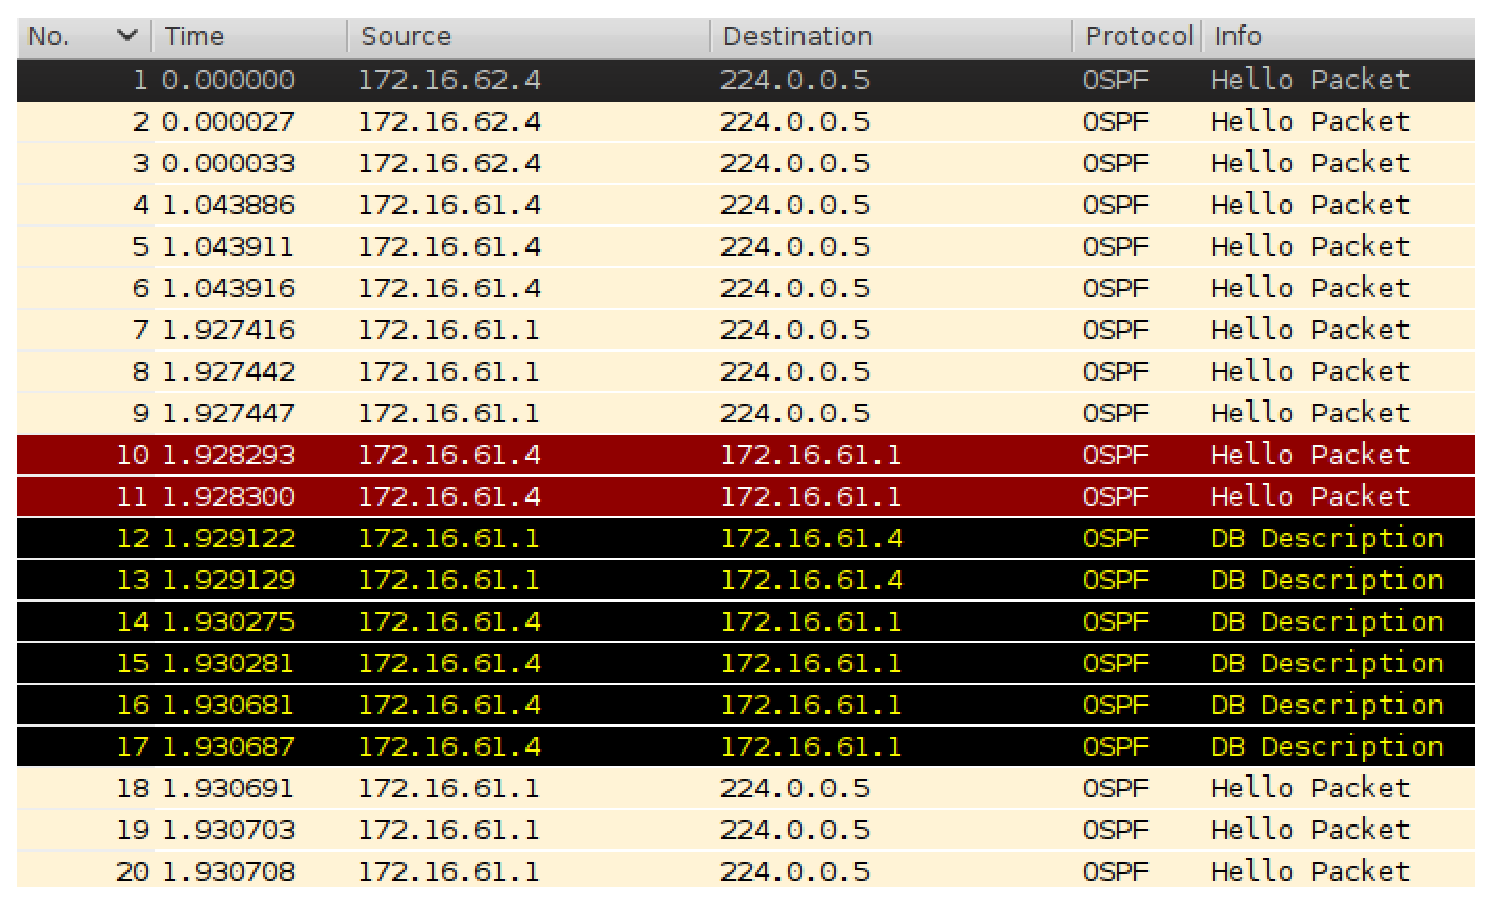
\includegraphics[width=6in]{cenario1-inicio1}
	\end{center}
	\caption{Tráfego interceptado entre os serviços de OSPF em funcionamento no router após ter sido iniciado e o GNU61 (Cenário 1).}
	\label{fig:cenario1-inicio1}
\end{figure}

\begin{figure}[htp]
	\begin{center}
		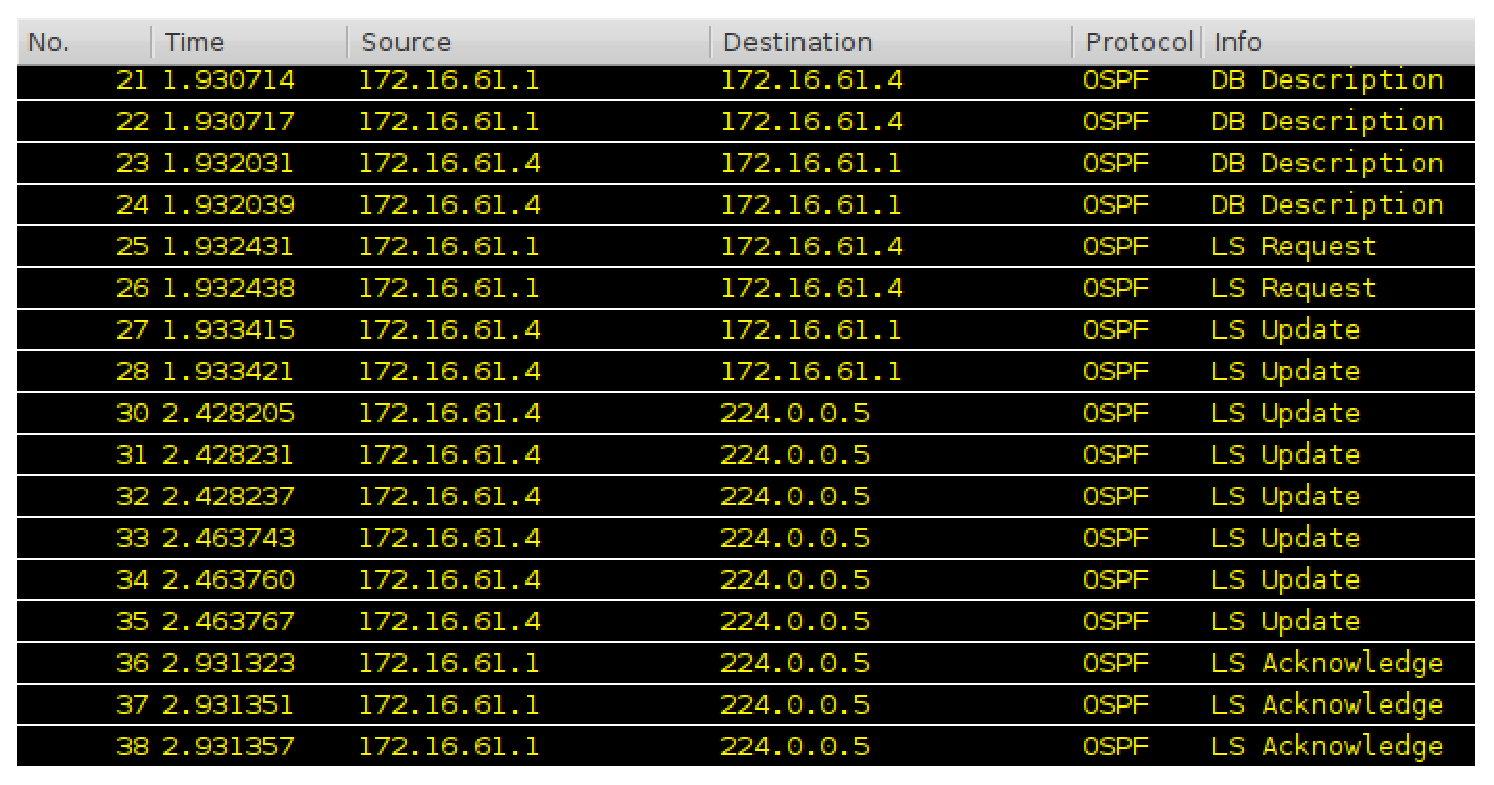
\includegraphics[width=6in]{cenario1-inicio2}
	\end{center}
	\caption{Continuação do tráfego interceptado entre o serviço OSPF do router e do recém iniciado serviço no GNU61.}
	\label{fig:cenario1-inicio2}
\end{figure}

\begin{figure}[htp]
	\begin{center}
		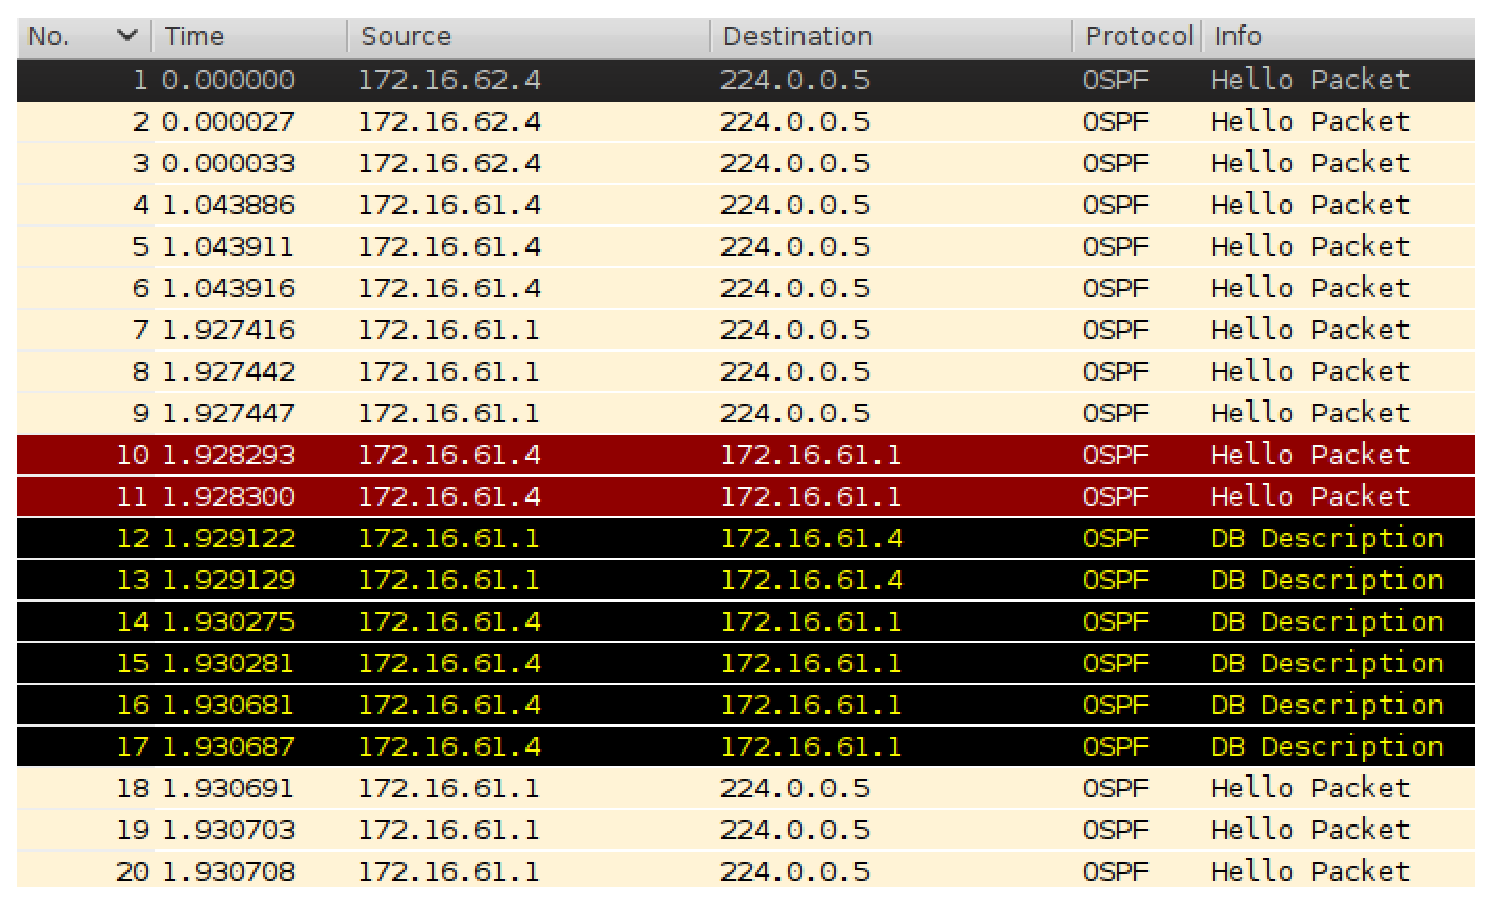
\includegraphics[width=6in]{cenario1-inicio1}
	\end{center}
	\caption{Tráfego interceptado a partir do momento em que toda a informação da rede ficou sincronizada em todos os serviços de OSPF da rede.}
	\label{fig:cenario1-fim}
\end{figure}

\section{Arquivos de log}

Na pasta logs anexada a este arquivo, podemos encontrar os logs e arquivos de
configuração capturados. Para este assumimos a seguinte convenção \verb gX  para
os Gnus (\verb X  representa o respectivo Gnu), \verb r6  para o router cisco, e
\verb s6  para o switch cisco. As pastas \verb logs/cY  representas os três
cenários indicados no guia (\verb Y  varia de 1 a 3 representando os cenários).
Já as pastas \verb logs/cY/trace_route  como o nome indica representa o
trace route de todos os componentes para todos os outros do sistema. Finalmente
as pastas \verb logs/conf/{gX,r6,s6}  mostram as configurações efetuadas no
sistema. Abaixo detalhamos os arquivos de cada pasta.

\begin{itemize}
	\item Para os logs em \verb-logs/cY-
		\begin{description}
			\item \verb *\_zebra  Representa o comando \verb-show ip route-.
			\item \verb *\_ospf  Representa o comando \verb-show ip ospf neighbor-.
		\end{description}
	\item Para os trace routes em \verb-logs/cY/trace_route-
		\begin{description}
			\item \verb {gX,r6}_{gX,r6}[.{61,62}]  Representa o trace route do
				elemento anterior ao \verb _  para o elemento posterior. A parte
				opicional que contém o \verb .  ilustra para o caso do \verb g2  e
				\verb r6  ondo o trace route pode ser feito a rede \verb 61  ou \verb 62 .
		\end{description}
	\item Para as configurações em \verb-logs/confs/gX-
		\begin{description}
			\item[zebra.conf] Apresenta a configuração do zebra no respectivo
				gnu.
			\item[ospfd.conf] Apresenta a configuração ospf no respectivo gnu.
		\end{description}
	\item Para as configurações em \verb-logs/confs/{r6,s6}-
		\begin{description}
			\item[running-config] Apresenta a configuração do router ou switch
				gerada com o comando \verb_show running-config_.
		\end{description}
\end{itemize}


\section{Referências}

SPAN: \url{http://www.cisco.com/en/US/products/hw/switches/ps708/products_tech_note09186a008015c612.shtml#terms}

\end{document}
